% 独自のコマンド

% ■ アブストラクト
%  \begin{jabstract} 〜 \end{jabstract}  :日本語のアブストラクト
%  \begin{eabstract} 〜 \end{eabstract}  :英語のアブストラクト

% ■ 謝辞
%  \begin{acknowledgment} 〜 \end{acknowledgment}

% ■ 文献リスト
%  \begin{bib}[100] 〜 \end{bib}


\newif\ifjapanese

\japanesetrue  % 論文全体を日本語で書く(英語で書くならコメントアウト)

\ifjapanese
  \documentclass[a4j,twoside,openright,11pt]{jreport} % 両面印刷の場合。余白を綴じ側に作って右起こし。
  %\documentclass[a4j,11pt]{jreport}                  % 片面印刷の場合。
  \renewcommand{\bibname}{参考文献}
  \newcommand{\acknowledgmentname}{謝辞}
\else
  \documentclass[a4paper,11pt]{report}
  \newcommand{\acknowledgmentname}{Acknowledgment}
\fi
\usepackage{thesis}
\usepackage{ascmac}
\usepackage{graphicx}
\usepackage{multirow}
\usepackage{url}
\bibliographystyle{jplain}

\bindermode  % バインダー用余白設定

\def\system{\textsf{SuprIME}}
\def\papertitle{\system: IMEによるテキスト編集機能の統合}

% 日本語情報(必要なら)
\jclass  {修士論文}                             % 論文種別
\jtitle    {\papertitle}    % タイトル。改行する場合は\\を入れる
\juniv    {慶應義塾大学大学院}                  % 大学名
\jfaculty  {環境情報学部}               % 学部、学科
\jauthor  {中園 翔}                       % 著者
\jhyear  {25}                                   % 平成○年度
\jsyear  {2013}                                 % 西暦○年度
\jkeyword  {IME,入力システム,テキスト編集,エディタ}     % 論文のキーワード
\jproject{増井俊之研究会} %プロジェクト名
\jdate{2014年1月}


\begin{document}

\ifjapanese
  \jmaketitle    % 表紙(日本語)
\else
  \emaketitle    % 表紙(英語)
\fi

\begin{abstract}
計算機上で様々なテキストエディタが利用されているが、
システムごとに編集方法や編集機能が異なっているのが不便である。
本論文では、各国語入力のためにOSに用意されているIME(Input Method Editor)機能を利用することにより、
あらゆるテキストエディタにおいて同じ操作によるテキスト編集を可能にする方法を提案する。
我々の手法を利用すると,異なるテキストエディタ上での編集操作が共通化されるだけでなく、
テキスト編集時に便利な様々な機能をあらゆるエディタで利用することが可能になる。
\end{abstract}
  % アブストラクト。要独自コマンド、include先参照のこと

\tableofcontents  % 目次
\listoffigures    % 図目次

\pagenumbering{arabic}


\section{はじめに}

計算機上でテキストを編集するために様々なテキストエディタが利用されている。
文書を作成するときはワープロを利用し、
メールを書くにはメールクライアントを利用し、
文字端末でのプログラム開発にはvimやEmacsを利用し、
IDEを利用した開発では付属のエディタを利用し、
ネット上でテキストを扱うにはブラウザのテキストフォームを利用するといったように、
場合に応じて様々なエディタが利用されている。

エディタの機能や操作体系はシステムごとに異なっているのが普通である。
ブラウザやワープロでテキストを1行消したい場合は
マウスで行全体を選択してから削除キーを押せばよいが、
vimでは「d」キーを2回タイプして消すことが多く、
EmacsではCtrl-Kキーがよく使われている。
Emacsに慣れたユーザがワープロ上でもCtrl-Kで行を消去したいと思っても、
そういう機能は用意されていないのが普通であるし、
機能拡張が可能なシステムを利用している場合でも、
操作体系を完全に同じにすることは難しい。
%
あらゆるエディタの操作を統一することは難しいが、
様々なエディタで共通に利用できるソフトウェア層を
ユーザとアプリケーションの間に置くことができれば
異なるエディタの編集操作をある程度共通化できる可能性がある。

現在のパソコンには IME(Input Method Editor) と呼ばれる文字入力機構が用意されており、
様々な言語のテキスト入力に利用されている。
IMEはエディタなどとは独立したソフトウェアであり、
ユーザのすべてのキー入力を受け取って
各国語に変換した結果をアプリケーションに送出する。
IMEはあらゆるアプリケーションで共通に利用されるので、
たとえば日本語入力用のIMEを利用すれば、
Emacs でもブラウザでも IDE でも同じ操作で日本語を入力できる。
IMEは一般には各国語入力のみのために利用されているが、
テキストの挿入/移動/削除といった編集操作もIMEが受け持つようにすれば、
様々なエディタ上で同じ操作で編集を行なうことが可能になる。
%
Mac上の様々なテキストエディタにおいて
同じキー操作でテキスト編集を可能にする{\system}システムについて述べる。



\section{{\system}使用例}

本章では{\system}を利用した様々な入力/編集作業の例を示す。

\subsection{日本語入力}

{\system}は、
MacRuby\footnote{
  RubyをMac用に拡張したもので、あらゆるMacのAPIをRubyから利用することができる。
}で記述された日本語IMEである「Gyaim\footnote{
 \textsf{https://github.com/masui/Gyaim}
}」に様々な編集機能を追加したものである。
%
図\ref{japaneseinput}は{\system}による日本語入力の例である。
IMEはアルファベット以外の文字を入力するときだけ有効にするのが普通であるが、
{\system}は、編集操作を行うために常に有効であることを想定して実装した。
そのため、英語入力と日本語入力の両方が可能である。

\begin{figure}[H]
\centerline{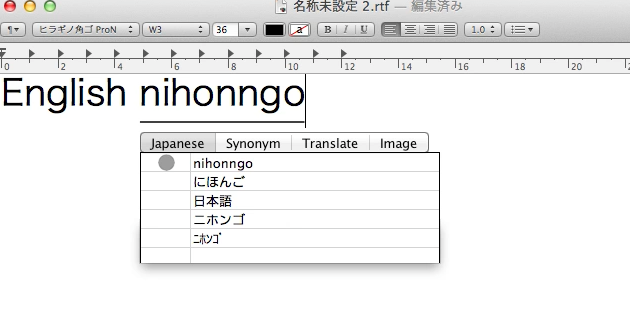
\includegraphics[width=70mm,bb=0 0 600 400]{figures/japanese.png}}
\caption{{\system}による日本語入力.}
\label{japaneseinput}
\end{figure}

\subsection{ブロック移動}

テキストの一部を別の場所に移動する操作は
テキストエディタの重要な機能のひとつであるが、
エディタによって操作方法が大きく異なっている。
たとえばEmacsでテキストを移動させたい場合は、
移動する領域をキー操作によって指定してから削除/コピーし、
カーソルを移動してからペーストするという手順を利用するのに対し、
ブラウザの編集領域でテキストを移動させたい場合は、
マウスで領域を指定した後で選択領域をドラッグして別の位置に移動することが多い。
このように、テキスト移動のような基本操作でもエディタごとに操作が異なっているのは不便であり、
操作ミスをしがちであるが、
{\system}を利用するとあらゆるエディタにおいて
同じ操作でテキストを移動することができる。

図\ref{move1}はMac OSに標準登載されている
「テキストエディット」でテキストを編集しているところである。

\begin{figure}[H]
\centerline{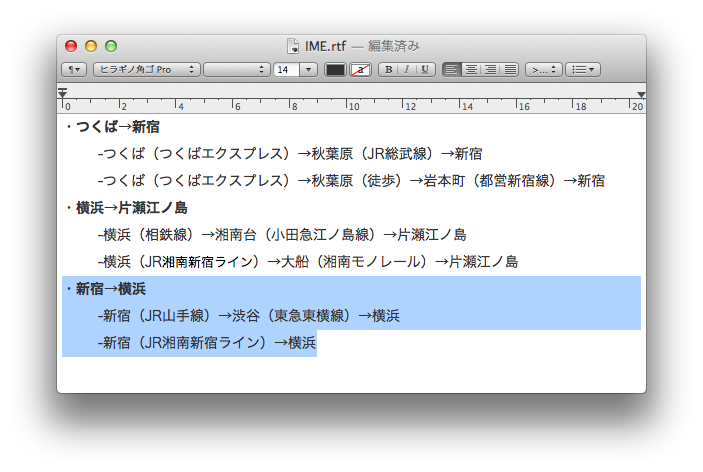
\includegraphics[width=70mm,bb=0 0 703 472]{figures/block2.png}}
\caption{ブロック移動前の状態.}
\label{move1}
\end{figure}

ここでShift+↑キーを押すとテキストは図\ref{move2}のように変化する。

\begin{figure}[H]
\centerline{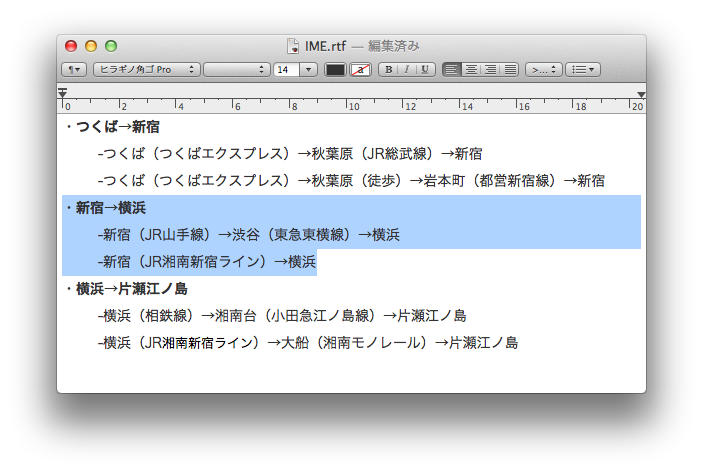
\includegraphics[width=70mm,bb=0 0 703 472]{figures/block3.png}}
\caption{Shift+↑キーを押した後の状態.}
\label{move2}
\end{figure}

図\ref{move3}はブラウザ上でGoogle Docsのテキストを編集しているところである。
ここでShift+↓キーを二度押すと、テキストは図\ref{move4}のように変化する。

\begin{figure}[H]
\centerline{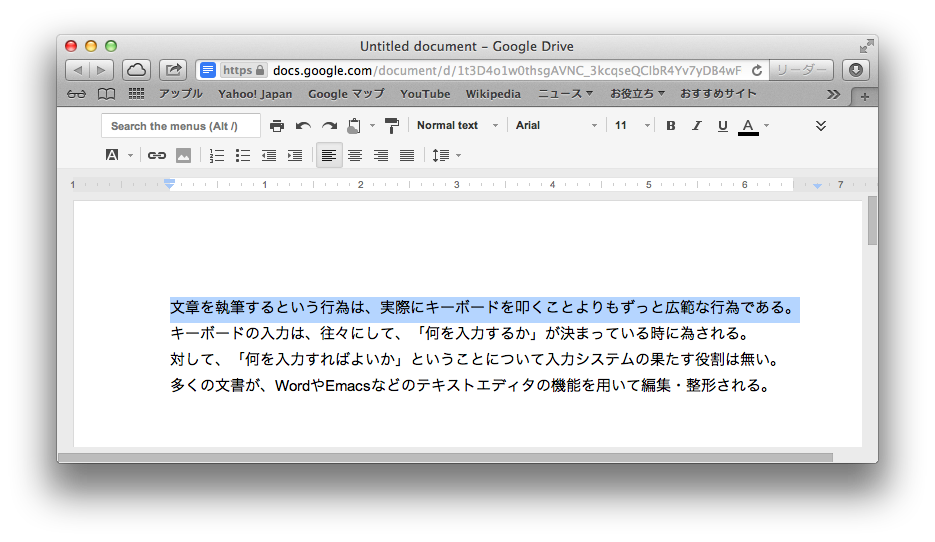
\includegraphics[width=70mm,bb=0 0 935 542]{figures/block4.png}}
\caption{ブロック移動前の状態.}
\label{move3}
\end{figure}

\begin{figure}[H]
\centerline{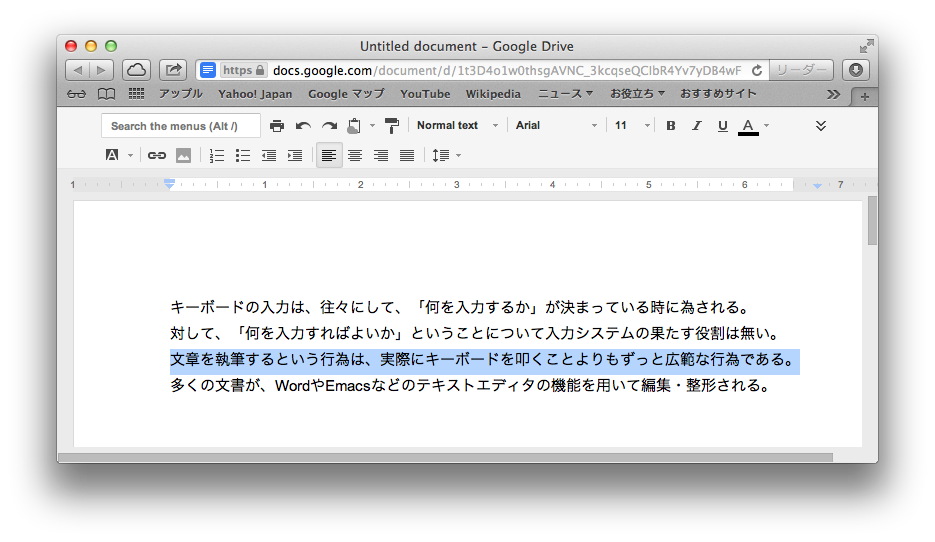
\includegraphics[width=70mm,bb=0 0 935 542]{figures/block5.png}}
\caption{キーを押した後の状態.}
\label{move4}
\end{figure}

このように、あらゆるエディタにおいて
Shift+矢印キーという共通の操作で
ブロック移動を行なうことができることがわかる。

\subsection{連続インデント}

前述したブロック移動は、インデントを調整する機能も備えている。
プログラミングを行なっている時だけでなく、
普通のテキストを編集している場合でも
行頭の空白やタブの量を調整するインデント処理は頻繁に行われるが、
自動的にインデントを行うエディタもあれば、
コマンドを打ち込まなければならないものもあり、
そのような調整機能を持っていないエディタも多い。
{\system}を利用すると、あらゆるエディタや入力フィールドでブロック移動と同時にインデントが自動で行われる。

図\ref{indent1}は、Xcode上でPythonプログラムを書いている例である。
Xcodeは、Objective-CやRubyなどの言語で自動インデントの機能を備えているが、Pythonには対応していない。
たとえば、図\ref{indent1}のようなテキストに対して
図\ref{indent2}のように移動させたいブロックを選択し、Shift+↓キーを入力することで、テキストは図\ref{indent3}のように変化する。

\begin{figure}[H]
\centerline{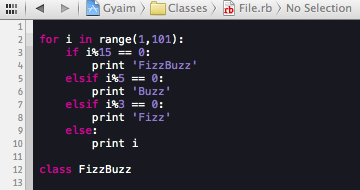
\includegraphics[width=70mm,bb=0 0 360 190]{figures/indent1.png}}
\caption{ブロック移動前の状態}
\label{indent1}
\end{figure}

\begin{figure}[H]
\centerline{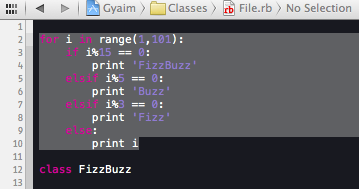
\includegraphics[width=70mm,bb=0 0 360 190]{figures/indent2.png}}
\caption{テキストを選択した状態}
\label{indent2}
\end{figure}

\begin{figure}[H]
\centerline{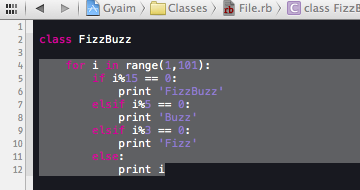
\includegraphics[width=70mm,bb=0 0 360 190]{figures/indent3.png}}
\caption{ブロック移動後の状態}
\label{indent3}
\end{figure}

このように、あらゆるエディタにおいて、ブロック移動を行う際に適切な空白とタブを自動で補完することができる。

\subsection{単語置換}

多くのエディタが単語の検索/置換機能を持っているが、
その操作方法はシステムごとに異なっている。
また、Webブラウザのテキスト編集領域では
通常検索/置換機能が用意されていない。
ブラウザに入力したテキストをエディタにコピーして編集操作を行うといった作業、
あるいはその逆といった作業を{\system}により共通化することができる。(???)

以下に{\system}による単語置換の例を示す。
あらかじめめ割り当てたファンクションキーを押すと、
図\ref{search1}のように{\system}の単語置換ウィンドウが起動する。

\begin{figure}[H]
\centerline{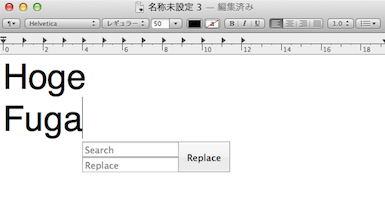
\includegraphics[width=70mm,bb=0 0 360 215]{figures/replace1.png}}
\caption{単語置換ウィンドウの例}
\label{search1}
\end{figure}

図\ref{search2}のように、入力語と置換語をテキストエリアに打ち込み、Replaceボタンを押すと、

\begin{figure}[H]
\centerline{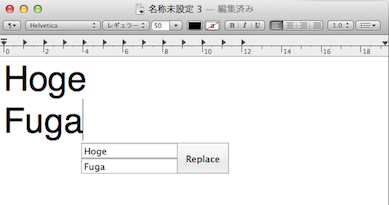
\includegraphics[width=70mm,bb=0 0 360 191]{figures/replace2.png}}
\caption{置換ウィンドウに単語を入力した例}
\label{search2}
\end{figure}


テキストは図\ref{search3}のように置換される。

\begin{figure}[H]
\centerline{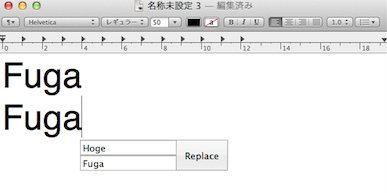
\includegraphics[width=70mm,bb=0 0 360 191]{figures/replace3.png}}
\caption{単語置換後の状態}
\label{search3}
\end{figure}

このように、あらゆるエディタ上で検索と置換が可能である。

\subsection{Emacs Lisp}
Emacsにおいてはlisp拡張を導入することでエディタの機能を拡張することが出来るが、これらのスクリプトをIME上に実装することで、他のエディタ上でもこれらの有用な拡張機能を動作させることができる。

以下に{\system}でDynamic Macro\cite{DynamicMacro}を実現した例を挙げる。
Dynamic Macroは、入力の繰り返しを自動化するEmacs拡張である。
図\ref{dynamic1}のように、ユーザの入力操作が繰り返しになっているとき、任意に設定したファンクションキーを押すと、テキストは図\ref{dynamic2}のように編集される。

\begin{figure}[H]
\centerline{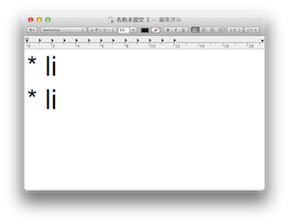
\includegraphics[width=80mm,bb=0 0 360 190]{figures/dynamic1.png}}
\caption{Dynamic Macro機能を使用する前のテキスト}
\label{dynamic1}
\end{figure}

\begin{figure}[H]
\centerline{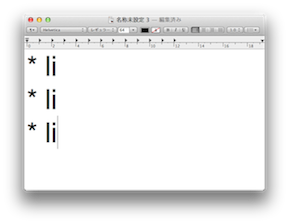
\includegraphics[width=80mm,bb=0 0 360 190]{figures/dynamic2.png}}
\caption{Dynamic Macro機能を使用した後のテキスト}
\label{dynamic2}
\end{figure}


以下は{\system}のDynamic Macro機能をブラウザのアドレスバー上で実行した例である。
図\ref{dynamic3}のように、ユーザの入力に"abc"が繰り返されているとき、任意に設定したファンクションキーを押すと、テキストは図\ref{dynamic4}のように編集される。

\begin{figure}[H]
\centerline{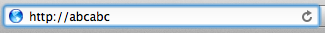
\includegraphics[width=70mm,bb=0 0 360 50]{figures/dynamic3.png}}
\caption{Dynamic Macro機能を使用する前のテキスト}
\label{dynamic3}
\end{figure}

\begin{figure}[H]
\centerline{
\includegraphics[width=70mm,bb=0 0 360 50]{figures/dynamic4.png}}
\caption{Dynamic Macro機能を使用した後のテキスト}
\label{dynamic4}
\end{figure}





\section{実装}
Gyaim は MacRuby で記述された Mac 用の IME であり、ソースが 500 行程度とコンパクトであるにもかかわらず、他の IME に見られない機能を実装しており、本論文のような実験も容易である。

\subsection{MacRuby}
MacRuby は、Mac 用のアプリケーションを開発するために拡張された Ruby 実行環境であり、Mac の Objective-C ライブラリを Ruby で扱うことが出来る。
Gyaim では、日本語などの入力を補助するフレームワークである InputMethodKit Framework を MacRuby から呼び出すことによって基本的な IME の機能を実装している。

\subsection{InputMethodKit Framework}
Mac OSX用に用意されたフレームワークであるInputMethodKit Frameworkは、全てのキー入力をハンドルする機能と、アクティブなアプリケーションに対してテキストを送出する機能を備えている。
一般的に、このような枠組みを利用して各国語用のIMEを開発する際には、エディタが編集機能のために用いる、ControlやCommandなどの修飾キーはハンドルしないのが普通であるが、Gyaimでは修飾キーに応じた編集操作を実現している。

しかし、ブロック移動やインデントの処理をあらゆる テキストエリアで行うためには、テキストフィールドに 入力されている全文をIMEが取得する必要があり、InputMethodKit はこの機能を備えていない。Gyaim では、AppleScript などを併用することによりこの問題を解決したが、実装には課題が残っている。

\section{議論}

\subsection{本手法の有用性}

パソコンやスマートフォンで利用されている様々なテキスト入力システムは
変換方式も使い勝手も全く異なっているのが普通になっているが、
単純で柔軟な入力方式を利用すると、
パソコンでもスマートフォンでもほぼ共通の入力を行なうことが可能である。
{\system}はこのような思想にもとづいて作成された IMEであるが、
本論文のような手法を取り入れることにより、
あらゆる機器において入力も編集もユニバーサルにすることが可能であろう。

\subsection{本手法の展望}

本論文ではテキストエディタに絞った説明を行なったが、IME はユーザ
のすべてのキー入力を直接受け取る窓口になっているため、編集と関係無いキー操作も IME に担当させることによってより幅広い計算機操作を実行することが
できる。たとえばシステム音量や画面の明るさをコントロールするにはシステ
ムに用意された特別のキーを使ったり、システムに用意されたショートカット
を利用したりすることが多いが、このようなものも IME から制御するようにし
ておけばシステム全体のショートカット設定などは不要になる。


また、文書の整形以外にも、IMEの実装によりテキスト入力を補助するという考え方はより広範な入力に当てはめることができる。
{\system}では、単語の言い換えを補助するために、図\ref{synonym}のように類語を入力することが出来る。

\begin{figure}[H]
\centerline{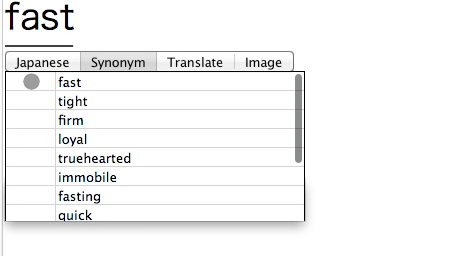
\includegraphics[width=70mm,bb=0 0 350 250]{figures/synonym.png}}
\caption{{\system}の類語変換機能の例。}
\label{synonym}
\end{figure}

図\ref{image1},\ref{image2}は{\system}の画像入力の例である。
ここでは、「知らない」という入力語句について画像を検索し、入力候補として表示している。
画像が埋め込めるテキストエリアであれば画像を埋め込み、そうでなければURLを入力する、といった機能も、IMEにより実装することができる。

\begin{figure}[H]
\centerline{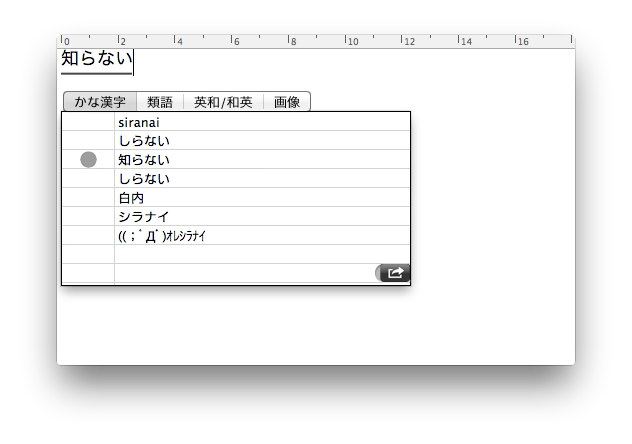
\includegraphics[width=70mm,bb=0 0 600 400]{figures/image1.png}}
\caption{{\system}で「知らない」という単語を入力した例。}
\label{image1}
\end{figure}

\begin{figure}[H]
\centerline{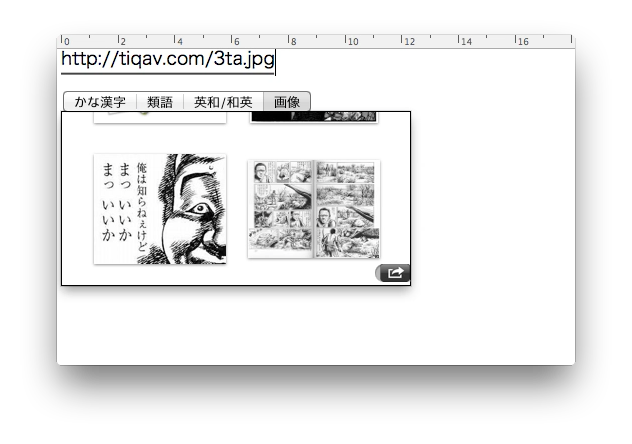
\includegraphics[width=70mm,bb=0 0 600 400]{figures/image2.png}}
\caption{{\system}の画像入力ウィンドウ。}
\label{image2}
\end{figure}

\subsection{本手法の限界}

IME はアプリケーションと独立に実装されているため、
現在のような実装ではアプリケーションの内部状態によって動作を変えたり、
アプリケーションの振る舞いを制御したりすることはできず、表に出ているテキストの編集操作しか
できない。 既存のシステム自体は変更せずに、皮をかぶせる形で機能を拡張す
る手法はある程度有用ではあるが、問題の根本的な解決が必要な場合には限界
がある。テキスト編集の場合は根本的に解決しなければならない問題は多くな
いので、本論文の手法はとりあえず有効だといえるが、根本的な解決のために
は、テキスト入力の枠組みであるIMEに加えて、各コンピュータがテキスト編集
のための枠組みを用意する必要があるだろう。

\subsection{コピー/ペーストと標準化}

Xerox PARCのLarry Teslerが70年代に発明した\cite{Tesler:CopyPaste}
「コピー/ペースト」は現在非常に普及しており、
ほぼすべてのアプリケーションにおいて同じ操作\footnote{
  Macの場合はCommand-CとCommand-V
}でテキストをコピーしたりペーストしたりできるようになっている。
つまりコピー/ペーストに関しては???章で述べたような問題がほぼ存在せず、
ユーザは混乱せずに様々なアプリケーション上でテキスト操作を行なうことが可能になっていることになる。
コピー/ペーストが標準化されているのに対し、
テキスト移動のような処理が全く標準化されていないのは不思議であるし、
そのことに不満を持っているユーザが多くないことも不思議である。
{\system}のような手法を利用することにより、
システム全体を統一的に利用できるようにする工夫が重用であろう。






\section{結論}


OSに標準装備されたIME機能を活用することにより,
様々なテキストエディタにおける入力/編集操作を共通化する手法を提案した.
IME機能はアプリケーションから独立しているため,
アプリケーション内のデータを操作することはできないが,
様々なアプリケーションにおける
入力/編集操作の多くの部分を共通化することができた.
%

テキストエディタの研究は長い歴史を持っているが\cite{texteditors.org},
近年はタブレットやモバイル環境における入力手法に関する研究%
\cite{Li:1lineKB}%
\cite{MacKenzie:H4Writer}%
\cite{Rick:VirtualKB}%
や特殊装置を使う文字入力装置に関する研究%
\cite{Dietz:PressureKB}%
\cite{Harrison:Skinput}%
\cite{Murase:CameraKB}%
\cite{Wigdor:TiltKB}
が主流になっており,一般的なテキストエディタを改善する研究は少ないようである.
テキストの入力や編集は計算機利用における最も重要な仕事のひとつであることは
間違いないので,
操作を簡単化/共通化するための優れた枠組みの開発は重要な課題だと考えられる.



\nocite{texteditors.org}
\nocite{Li:1lineKB}
\nocite{MacKenzie:H4Writer}
\nocite{Rick:VirtualKB}
\nocite{Dietz:PressureKB}%
\nocite{Harrison:Skinput}%
\nocite{Murase:CameraKB}%
\nocite{Wigdor:TiltKB}

\begin{acknowledgment}

このテンプレートを改造するにあたって、@kurokoboとインターネット上のいくつかの修士論文などを参考にしました。感謝いたします。

\end{acknowledgment}
  % 謝辞。要独自コマンド、include先参照のこと

\begin{bib}[100]
% BibTeXを使う場合
\bibliography{paper}

\end{bib}
  % 参考文献。要独自コマンド、include先参照のこと
\appendix
\chapter{付録の例}

付録を無理矢理出力させるため、てきとうなことを書く。

\section{ほげ}

コマンドは本文と一緒。

\subsection{ふー}

本文と一緒。

\section{ほげほげ}

本文と一緒。

\subsection{ふーふー}

本文と一緒。
    % 付録

\end{document}
